\documentclass[../main.tex]{subfiles}
% Subsección 4.2 del texto
\begin{document}
\subsection{Exploring the democracy variable}
\begin{figure}[H]
\centering
\fbox{
\begin{minipage}{\textwidth}
    \vspace{0.1cm}
    \caption{Political Regime (Democracy Score) Choropleth Map}
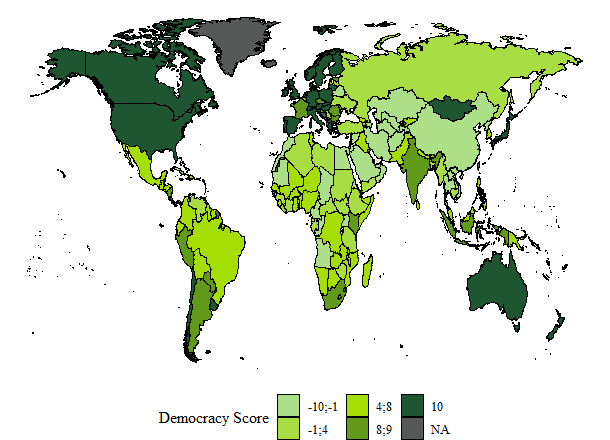
\includegraphics{../figures/maps/dem_map.png}
 \label{fig:2}
 \textit{Note:} Data from the PolityIV Project and Wimmer and Min (2006) compiled by Our World in Data (2015). In countries where no data was available, this graph set a democracy score based on political regime scores included in the V-Dem Dataset, also compiled by Our World in Data (2015); see Appendix \hyperref[sec:A]{A} for the countries that used this source as a base value. Elaborated by the Author.
\end{minipage}
    }
\end{figure}
As observed in the previous models, the degree in which a regime is democratic keeps a negative relationship with migrant stocks, which does not make sense with the literature or with common intuition. It would be expected that a more democratic regime also entails better institutions, easier transitions to labor markets, among others, thus more desirability as a long-term destination. Besides, \textcite{Beine.2008} suggest democratic countries are more desirable for migrants, since they are more likely to respect property rights.

However, democracy and migrant stocks are negatively related in the sample, even when accounting for the high migration in the MENA region, as well as desires to influence migrant stocks through policy. This counterintuitive sign may still happen since statistical relationships there seem to work in a different way. Refugee crises, which by construction cause higher migrant stocks, combined with autocratic regimes may be causing this sign. Figure \ref{fig:1} shows that there are higher migrant stocks here and Figure \ref{fig:2} shows that this region also presents low levels of democracy. This could be a significant limitation for this empirical approach since the different statistical relationships between regions confound the estimation process. In this section, I further explore this limitation with the models in Table \ref{tab:2}.

The model in the first column of Table \ref{tab:2} features an interaction between democracy and the MENA dummy, as specified in Equation \ref{eqn:2}. Now the $x_j$  include the $k$ covariates in the model in column 6 of Table \ref{tab:1}, except unemployment and the policy dummies.
\begin{equation}
IMS=\beta_0+\beta_1 (\text{democracy}) + \beta_2 (MENA)+ \beta_{3} (\text{democracy} \cdot MENA)+\sum_{j=1}^k \beta_j\hspace{0.05cm} x_j+u
    \label{eqn:2}
\end{equation}

This would imply that the effect of democracy is different for countries inside MENA. The results show that more democratic regimes for countries \textit{not} in this region still are supposed to have lower levels of migration.  However, the magnitude of the democracy coefficient in the model in column 1 of Table \ref{tab:2} is smaller than all democracy coefficients in Table \ref{tab:1}, which shows that its effect is less negative outside MENA. The negative sign on the interaction term implies that more democratic regimes inside this region face even lower levels of migrants. The model increased its explanatory power, which means that allowing for a special effect of democracy inside MENA is a better fit to the data. 
\subfile{../tables/table2}
\clearpage
In the model in the second column of Table \ref{tab:2}, I account for another interaction of the democracy variable, this time with income per capita, besides from the interaction seen in Equation \ref{eqn:2}.
\begin{equation}
\begin{split} % Para partir ecuaciones largas en dos o más líneas, utiliza operador de alineación &
IMS=&\beta_0+\beta_1 (\text{democracy}) + \beta_2 (MENA)+ \beta_{3} (\text{democracy} \cdot MENA)+\beta_4 \ln (GDP_{PC}) + \\ 
     &\beta_5 [ \ln (GDP_{PC}) \cdot \text{democracy}]+\sum_{j=1}^k \beta_j\hspace{0.05cm} x_j+u 
     \end{split}
    \label{eqn:3}
\end{equation}

Having both MENA and income interactions would imply that the partial effect of democracy is now more complex, as shown below. 
\begin{equation}
    \frac{\partial \ IMS}{\partial \ \text{democracy}} = \beta_1+\beta_3 MENA +\beta_5 \ln (GDP_{PC})
    \label{eqn:4}
\end{equation}

The first interaction is no longer significant, which suggests that there is not a special effect of democracy for MENA countries, once accounting for the income interaction. Now, the counterintuitive relationship has to do with income and democracy: supposedly more democratic and richer countries are associated with reductions in migrant stocks. These variables are jointly significant, and at the median level of income in the dataset, the partial effect of democracy on migrant stocks is still practically significant. 

Once again, the circumstances in MENA might still be an important limitation for an unbiased estimation of partial effects. In this region, but mostly in the Middle East, there are rich oil-exporting countries, which tend to have low democracy scores and very high-income per capita. As all countries in MENA, they have high migrant stocks, and the estimation process may confound these as causality relationships.

Income and democracy inside countries that do not belong to MENA are positively related, whereas the same relationship is negative inside MENA, as seen in Figure \ref{fig:3}, panel \ref{fig:3a}.  This could partly explain the sign on the second interaction term seen in the model in column 2 of Table \ref{tab:2}. Furthermore, inside MENA, richer countries are mostly petroleum exporters, as seen in panel \ref{fig:3b} of Figure \ref{fig:3}: a country that has higher oil rents tends to be less democratic.
\begin{figure}[H]
\centering
\fbox{
\begin{minipage}{\textwidth}
\vspace{0.1cm}
\caption{Democracy scores by income per capita and oil rents}    
    \label{fig:3}
    \begin{subfigure}[b]{0.49\textwidth}
    \centering
    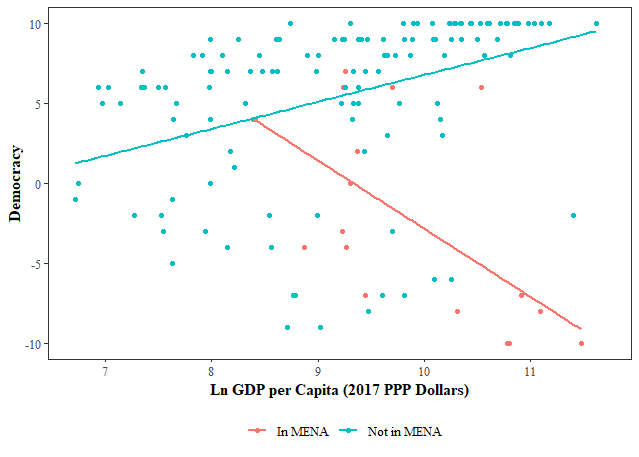
\includegraphics[scale=0.49]{../figures/scatter/dem_gdp.png}
    \caption{Democracy by GDPPC, in and out of MENA}
    \label{fig:3a}
    \end{subfigure}
    \hfill
     \begin{subfigure}[b]{0.49\textwidth}
     \centering
     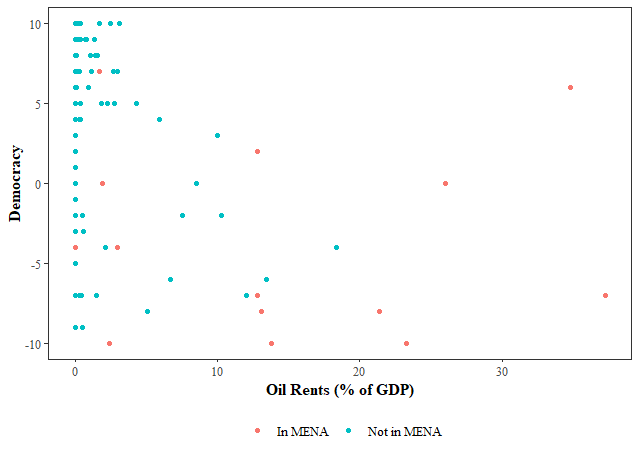
\includegraphics[scale=0.49]{../figures/scatter/dem_oilr.png}
    \caption{Democracy by oil rents, in and out of MENA}
    \label{fig:3b}
    \end{subfigure}
        \textit{Note:} Political stability and absence of violence data from the World Governance Indicators of the World Bank. Covariate data from the World Bank and Our World in Data (2015). Not all points in the graphs are used in the samples for regressions, as some countries have missing data on other covariates. Elaborated by the Author.
    \end{minipage}
    }
\end{figure}

High migration stocks in this region due to instability are likely to bias the estimation of coefficients, especially those involving democracy scores; this limits the identification strategy. The limitation may be born from the counterintuitive statistical relationships in some countries, which probably arise from events that do not happen elsewhere. Very high migration stocks are seen in authoritarian and high-income per capita nations, which gives the sense that these are desirable qualities for a migrant, when it should be the contrary, at least according to the literature. This can also be seen in Figure \ref{fig:4}. Outside MENA, the democracy variable is positively correlated with migrant stocks, which is coherent, but the correlation is small which may signal little importance of democracy on migrant stocks. Panel \ref{fig:4b} of Figure \ref{fig:4} shows that the relationship with income per capita is much stronger in MENA, suggesting the variable plays a more important role here in determining migrant stocks, relative to the rest of the world. 

The model in column 3 of Table \ref{tab:2}, now includes an interaction term between the MENA dummy and income per capita, as represented in Equation \ref{eqn:5}, to evaluate the fit of the data on a model based on the points made before. 
\begin{figure}[H]
\centering
\fbox{
\begin{minipage}{\textwidth}
\vspace{0.1cm}
\caption{International migrant stock (\% of total population) by democracy score and income per capita}    
    \label{fig:4}
    \begin{subfigure}[b]{0.49\textwidth}
    \centering
    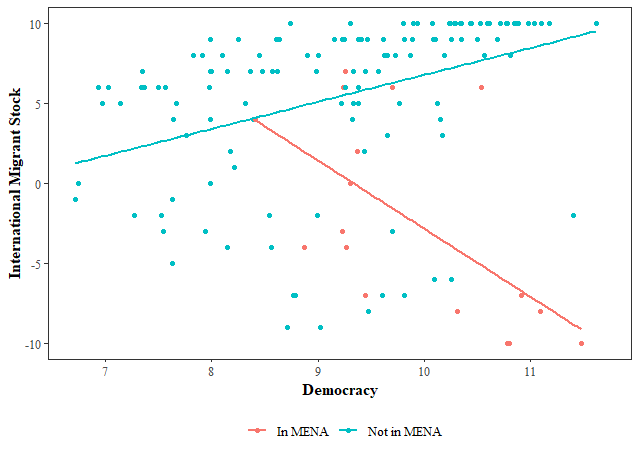
\includegraphics[scale=0.49]{../figures/scatter/ims_dem.png}
    \caption{IMS by democracy score, in and out of MENA}
    \label{fig:4a}
    \end{subfigure}
    \hfill
     \begin{subfigure}[b]{0.49\textwidth}
     \centering
     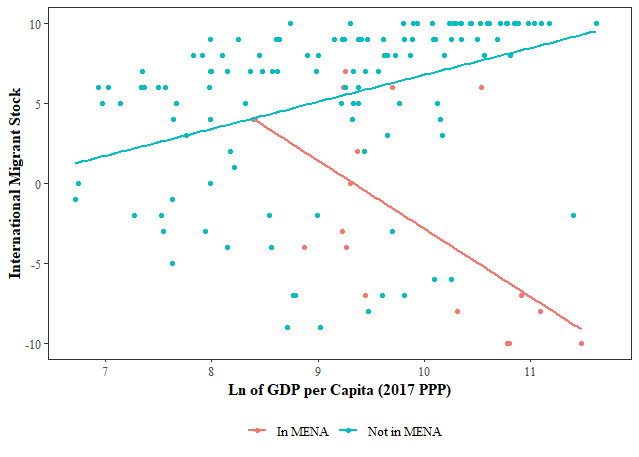
\includegraphics[scale=0.49]{../figures/scatter/ims_gdp.png}
    \caption{IMS by income per capita, in and out of MENA}
    \label{fig:4b}
    \end{subfigure}
      \textit{Note:} Data from the World Bank and Our World in Data (2015). Not all points in the graphs are included in the samples for regressions, as some countries have missing data on the other covariates. Elaborated by the Author.
    \end{minipage}
}
\end{figure}
\begin{equation}
\begin{split}
IMS=&\beta_0+\beta_1 (\text{democracy}) + \beta_2 (MENA)+ \beta_{3} (\text{democracy} \cdot MENA)+\beta_4 \ln (GDP_{PC}) + \\ 
     &\beta_5 [ \ln (GDP_{PC}) \cdot \text{democracy}]+\beta_6 [ \ln (GDP_{PC}) \cdot MENA]+\sum_{j=1}^k \beta_j\hspace{0.05cm} x_j+u 
     \end{split}
    \label{eqn:5}
\end{equation}

The results show that the terms involving democracy are not individually significant, however, all the democracy terms are jointly significant at the 99\% level. The interaction between income and democracy still has a counterintuitive sign, as it suggests that richer, more democratic countries see reductions in migrant stocks, as shown in the previous models. However, more democratic countries inside MENA, other things equal, see higher migrant stocks, which is intuitive. At the median level of income, the partial effect of democracy on migrant stocks is negative for countries both in and out of MENA, as the magnitude in the MENA dummy and democracy is not large enough to offset the negative coefficient on the income and democracy interaction. This partial effect will become more negative for richer countries, as seen by the sign on the income and MENA interaction term. 

The results also show a stronger relationship of income per capita within MENA, represented by the new interaction term. A 1\% increase in income per capita has a positive effect on migrant stocks around the world, as seen in all previous models. The model in the third column of Table \ref{tab:2} shows that the same 1\% increase in income per capita is related with a much bigger increase in migrant stocks inside MENA. This is consistent with Figure \ref{fig:4}, panel \ref{fig:4b}, where the slope in the relationship of income per capita and migrant stocks is higher for MENA countries. All the terms involving the income variable are jointly significant, and their inclusion seems to eliminate the significance of democracy in the model. This could be seen as more consistent than the previous relationships found between democracy and migration, however, the literature has not found a higher income effect on migration found only in MENA countries. 

In the model in column 4 of Table \ref{tab:2}, I replace the MENA region by another dummy variable, which equals 1 for rich oil exporting countries\footnote{See Appendix \hyperref[sec:A]{A} for details on the conditions for a country to be considered as a ``rich oil exporting country'' in this dataset.} (ROEC). The model is specified below:
\begin{equation}
\begin{split}
IMS=&\beta_0+\beta_1 (\text{democracy}) + \beta_2 (ROEC)+ \beta_{3} (\text{democracy} \cdot ROEC)+\beta_4 \ln (GDP_{PC}) + \\ 
     &\beta_5 [ \ln (GDP_{PC}) \cdot \text{democracy}]+\beta_6 [ \ln (GDP_{PC}) \cdot ROEC]+\sum_{j=1}^k \beta_j\hspace{0.05cm} x_j+u 
     \end{split}
    \label{eqn:6}
\end{equation}

The rich oil exporting countries dummy along with its interaction terms is jointly significant as a replacement for the MENA dummy seen in the model in column 3 of Table \ref{tab:2}.  Terms including democracy are jointly significant to this model, although most are not so in their own. A rich oil exporting country that is more democratic sees reductions in its migrant stock. Besides, a more democratic and higher income country features a relatively small decrease in its migrant stock. A rich oil exporting country with higher income per capita is associated with higher levels for the response variable. Still, the limitation is still present in the empirical method, but it directs attention toward rich oil exporters, which are mostly located in the MENA region.  The ethnic diversity variable loses significance when considering this new dummy. 
\begin{figure}[H]
\centering
\fbox{
\begin{minipage}{\textwidth}
\vspace{0.1cm}
\caption{Political stability and absence of violence (PSA) by income per capita and democracy score}    
    \label{fig:5}
    \begin{subfigure}[b]{0.49\textwidth}
    \centering
    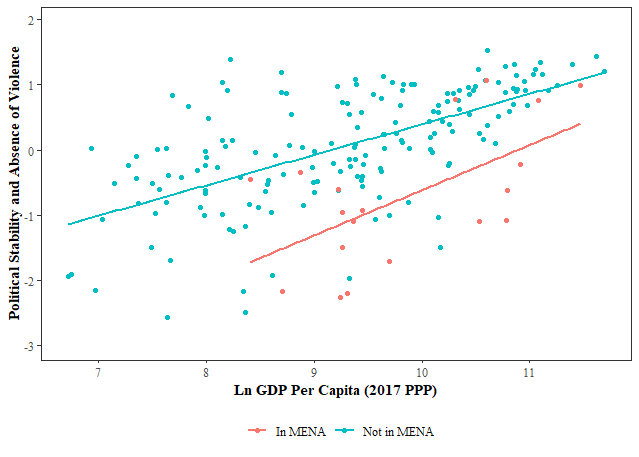
\includegraphics[scale=0.49]{../figures/scatter/psa_gdp.png}
    \caption{PSA by income per capita, in and out of MENA}
    \label{fig:5a}
    \end{subfigure}
    \hfill
     \begin{subfigure}[b]{0.49\textwidth}
     \centering
     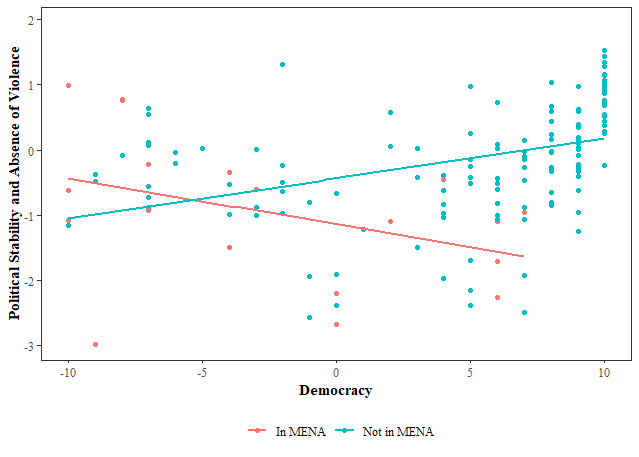
\includegraphics[scale=0.49]{../figures/scatter/psa_dem.png}
    \caption{PSA by democracy score, in and out of MENA}
    \label{fig:5b}
    \end{subfigure}
    \textit{Note:} Political stability and absence of violence data from the World Governance Indicators of the World Bank. Covariate data from the World Bank and Our World in Data (2015). Not all points in the graphs are used in the samples for regressions, as some countries have missing data on other covariates. Elaborated by the Author.
    \end{minipage}
    }
\end{figure}

It would seem that migrants in MENA are concentrated on the higher income per capita countries, and not in the more democratic ones. Migrants here could be looking for economic stability and peacefulness as a priority. Using the World Bank’s political stability and absence of violence indicator, panel \ref{fig:5a} in Figure \ref{fig:5} shows that in all the world, more stable and peaceful countries are also richer. On the other hand, panel \ref{fig:5b} shows that democracy inside MENA is fragile. Democratic regimes here are mostly correlated with more instability and violence. This could be the reason why the interaction terms in the model in column 4 of Table \ref{tab:2} have these signs: more democratic countries inside MENA see less stability and consequently less migration.

Yet, this is still no definitive justification on democracy being a repellent of migration, or a source for instability. It is difficult to infer causality for all these relationships due to the possibility of endogeneity or misspecification in the models. This further supports the idea that this empirical method may be limited, partly because of the relationships inside the MENA region, especially those surrounding democracy. In order to acquire an intuitive coefficient, which captures the benefits of democracy such as stability, peace, freedom of speech, participation in government, there might be a need for variables which are unobservable, such as the ‘true’ policy motivation of governments, the relative ‘fragility’ of democracy rather than the type of regime, among others.

The model in the fifth column of Table \ref{tab:2} further shows this by repeating the model in column 3 of Table \ref{tab:2}, but now eliminating the countries inside the MENA region, and its dummy. This model is specified as follows:
\begin{equation}
    IMS=\beta_0+\beta_1 (\text{democracy}) + \beta_2 \ln (GDP_{PC})+\beta_3[\ln (GDP_{PC}) \cdot \text{democracy}]+\sum_{j=1}^k \beta_j\hspace{0.05cm} x_j+u
    \label{eqn:7}
\end{equation}

Here, the partial effect of democracy depends only on the value of income per capita, unlike the more complex effect in Equation \ref{eqn:4},  as follows: 
\begin{equation}
    \frac{\partial \ IMS}{\partial \ \text{democracy}} = \beta_1+\beta_3 \ln (GDP_{PC})
    \label{eqn:8}
\end{equation}

The democracy terms, are jointly significant even if not individually so, and hold the same signs as before. However, the magnitude of the partial effect of democracy, at the median level of income is smaller than in the models that were shown before. This suggests that democracy causes a smaller negative effect on migrant stocks when leaving out the MENA countries, as I had hypothesized before. The signs on the control variables are similar, and ethnic diversity sees significance again. 
\begin{figure}[H]
\centering
\fbox{
\begin{minipage}{\textwidth}
    \vspace{0.1cm}
    \caption{Historical Index of Ethnic Fractionalization Choropleth Map}
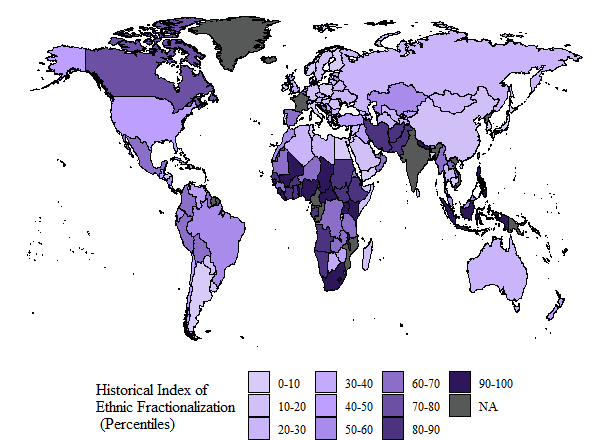
\includegraphics{../figures/maps/hief_map.png}
 \label{fig:6}
\textit{Note:} Data from the Harvard Dataverse. See Appendix \hyperref[sec:A]{A} for information on units of measurement for this variable. Elaborated by the Author.
\end{minipage}
    }
\end{figure}

Figure \ref{fig:6} shows how some MENA countries have 'medium' values of ethnic diversity and, as seen in Figure \ref{fig:1}, also have very high migrant stocks. The returning significance that ethnic diversity presents in the model in the fifth column of Table \ref{tab:2} would be expected when dropping MENA countries, as now migrants are concentrated more in countries that are more ethnically diverse, as both the literature and the models in Table \ref{tab:1} show. The estimation process is somewhat less limited, at least for the ethnic diversity index, when leaving out MENA countries.

The model in column 6 of Table \ref{tab:2}, also repeats the model in column 5 of Table \ref{tab:2} but now only considers countries in the western hemisphere\footnote{See Appendix \hyperref[sec:C]{C} for a list of countries included in this restricted model.}. In this new sample, there are some particular details about the effect of income and democracy on migrant stocks; the other variables, except ethnic diversity, keep their sign and significance. The standard error on the ethnic diversity coefficient increases for this reduced sample, which would be expected as it is more difficult to estimate partial effects with low variability in the regressors; Figure \ref{fig:6} shows that in western countries there is less variability of ethnic diversity. 

All terms involving income are jointly significant, yet its partial effect is increasing in democracy, as it can be seen in Equation \ref{eqn:9}. 
\begin{equation}
    \frac{\partial IMS}{\partial \ln({GDP_{PC}})}= \beta_2 + \beta_3 \text{democracy}
    \label{eqn:9}
\end{equation}

Results for this model in Table \ref{tab:2} show that there are positive effects of income per capita on migrant stocks \textit{only} for some kinds of anocracies. Anocracies, while not exactly a fully autocratic regime, do show instability: \enquote{characterized by institutions and political elites that are far less capable of performing fundamental tasks and ensuring their own continuity [...] a middling category rather than a distinct form of governance} \parencite[p.30]{Marshall.2017}. Only some anocracies have positive partial effects for income per capita, as the scores for anocracies range from -5 to 5, and the cutoff value for positive partial effect is about 4.40. Richer countries, but at lower values of democracy, actually see reductions of migrant stocks. This could suggest consistency with the literature on democracy: institutions, freedom of speech and participation in the political processes are important too; a migrant does not only decide on destination based on relative richness of countries. 

Terms involving democracy are also jointly significant; I keep the interaction term seen in Equation \ref{eqn:7}. Other things equal, countries which are richer and more democratic have higher migrant stocks, however, the partial effect of democracy, also represented through Equation \ref{eqn:8}, does not turn positive until income per capita reaches its 58\textsuperscript{th} percentile (about 28 thousand 2017 PPP dollars), as seen in Figure \ref{fig:7}, panel \ref{fig:7a} below. Democratic countries only see high migrant stocks when they have high values of income per capita, otherwise, they see reductions in the response variable. This supports the idea of a possible `balance' that migrants look for between income per capita and democracy. Figure \ref{fig:7} shows the partial effects of democracy and income per capita for different values of income per capita and democracy, respectively. The $x$-axis intercepts for each straight line represent the cutoff values for which the partial effects start to turn positive.

\begin{figure}[H]
\centering
\fbox{
\begin{minipage}{\textwidth}
\vspace{0.1cm}
\caption{Partial Effects (PE) of Democracy and Income Per Capita on International Migrant Stocks in the Western Hemisphere}        \label{fig:7}
    \begin{subfigure}[b]{0.49\textwidth}
    \centering
    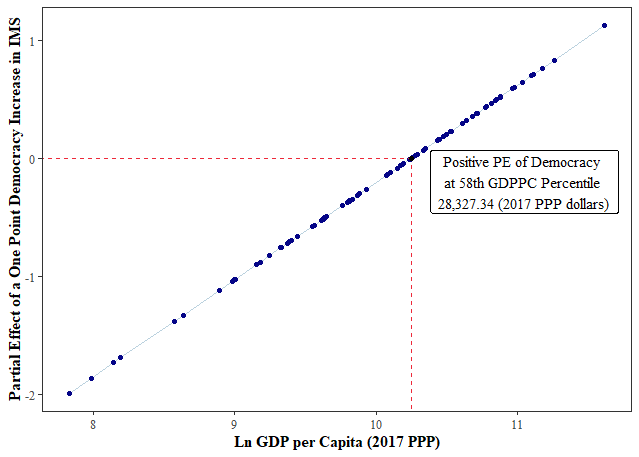
\includegraphics[scale=0.49]{../figures/scatter/pe1.png}
    \caption{Partial effect of democracy by $\ln(GDP_{PC})$ value}
    \label{fig:7a}
    \end{subfigure}
    \hfill
     \begin{subfigure}[b]{0.49\textwidth}
     \centering
     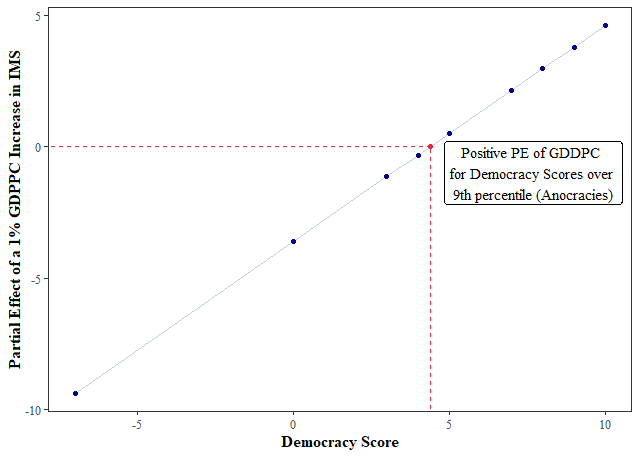
\includegraphics[scale=0.49]{../figures/scatter/pe2.png}
    \caption{Partial effect of \ $\ln{(GDP_{PC}})$ by democracy score}
    \label{fig:7b}
    \end{subfigure}
    \textit{Note:} The vertical axis shows the change in international migrant stock due to a 1\% or point increase of income per capita or democracy, respectively. Since there are interaction terms between these variables, these partial effects depend on the values of income per capita and democracy, respectively. These partial effects values $\partial IMS/\partial \text{democracy}$ and $\partial IMS/\partial \ln(GDP_{PC})$, plotted in the $y$-axes, are derived from Equation \ref{eqn:7}, and represented in Equations \ref{eqn:8} and \ref{eqn:9}. These are estimated through the model in column 6 of Table \ref{tab:2}. The $x$-axis values for each graph are those found in the sample for the Western Hemisphere. Elaborated by the Author. 
    \end{minipage}
    }
\end{figure}



\end{document}